\documentclass[conference]{IEEEtran}
\IEEEoverridecommandlockouts
% The preceding line is only needed to identify funding in the first footnote. If that is unneeded, please comment it out.
\usepackage{cite}
\usepackage{amsmath,amssymb,amsfonts,amsthm}
\usepackage{algorithmic}
\usepackage{graphicx}
\usepackage{textcomp}
\usepackage{xcolor}
\usepackage{minted}
\RecustomVerbatimEnvironment{Verbatim}{BVerbatim}{}
\usepackage{colortbl}
\usepackage{stfloats}
\usepackage{cite}  % converts [1],[2] to [1,2]
\usepackage{multicol}
\usepackage{mathtools}
\usepackage{hyperref}
\usepackage{subfiles}


\makeatletter
\def\@citex[#1]#2{\leavevmode
\let\@citea\@empty
\@cite{\@for\@citeb:=#2\do
{\@citea\def\@citea{,\penalty\@m\ }%
\edef\@citeb{\expandafter\@firstofone\@citeb\@empty}%
\if@filesw\immediate\write\@auxout{\string\citation{\@citeb}}\fi
\@ifundefined{b@\@citeb}{\hbox{\reset@font\bfseries ?}%
\G@refundefinedtrue
\@latex@warning
{Citation `\@citeb' on page \thepage \space undefined}}%
{\@cite@ofmt{\csname b@\@citeb\endcsname}}}}{#1}}
\makeatother

\renewcommand{\qedsymbol}{$\blacksquare$}

\newtheorem{thm}{Theorem}[section]
\newtheorem{lem}[thm]{Lemma}
\newtheorem{prop}[thm]{Proposition}
\newtheorem{cor}{Corollary}
\newtheorem{conj}{Conjecture}[section]
\theoremstyle{definition}
\newtheorem{defn}{Definition}[section]
\newtheorem{exmp}{Example}[section]
\newtheorem{rem}{Remark}

\def\BibTeX{{\rm B\kern-.05em{\sc i\kern-.025em b}\kern-.08em
    T\kern-.1667em\lower.7ex\hbox{E}\kern-.125emX}}

\begin{document}
\title{Finitely Presented Group Construction from Turing Machine}

\author{\IEEEauthorblockN{Maksym Shamrai}
\IEEEauthorblockA{\textit{Saint Petersburg State University}\\
St. Petersburg, Russia \\
vortmanmax@gmail.com}
\and
\IEEEauthorblockN{Semyon Grigorev}
\IEEEauthorblockA{\textit{Saint Petersburg State University}\\
\textit{JetBrains Research}\\
St. Petersburg, Russia \\
s.v.grigoriev@spbu.ru \\
semyon.grigorev@jetbrains.com}
}

\maketitle

\begin{abstract}
A study of formal languages showed there are open problems that rather difficult to solve involving traditional combinatorial methods. In this paper, we try to bring group theory methods into play by developing an algorithm, which had been described by Sapir, Birget, and Rips, and constructs a presentation of a finitely presented group by a given Turing machine. Also, we obtained an injective mapping from an alphabet of the Turing machine language into a word problem of the corresponding group. The algorithm can be used to further study the classification of formal languages in terms of well-known classes of groups, highlight signs of belonging to a particular class, and apply the algebraic methods to formal languages. Generally, we try to bring new approach to analyze formal languages by group theory. 
\end{abstract}

\begin{IEEEkeywords}
Turing machine, symmetric Turing machine, S-machine, group presentation, group theory, word problem, formal languages, Haskell
\end{IEEEkeywords}

\section{Introduction}

%Formal languages is a field of math which gain widespread use in such areas like
Formal languages are the theoretical foundation of system programming, namely the development of translators and static analyzers, through lexical, syntactic, and semantic analysis.
The formal language analysis approach has begun new development in the 50s of the last century~\cite{chomsky1, chomsky2}.
During this time, it found application not only in areas directly related to programming but, among other things, in the analysis of graph data models~\cite{Hellings2015QueryingFP, Azimov}, which are used,
for example, in bioinformatics~\cite{Huber2007} and social networks~\cite{scott1988social}.

Development entails new theoretical problems and challenges.
Several of them are associated with the advent of conjunctive~\cite{ConjGrammars} and Boolean language~\cite{BoolGrammars} classes.
The first and most important issue concerns the bounds of Boolean grammars.
The limitations of the expressive power of conventional context-free grammars are fairly well known. There are direct methods for proving the unrepresentability of certain languages,
such as the pumping lemmas and its variants~\cite{pumpingLemma}, which show that some languages
cannot be generated by a context-free and regular grammars. On the contrary, there are no methods
for proving the unrepresentability of languages by Boolean grammars, and this
is the main gap in the knowledge of these grammars. Similarly,
such methods are not known for conjunctive grammars~\cite{OKHOTIN201327}.

Recently, there has been a tendency to shift the direction of methods of studying formal languages.
Researchers are moving away from combinatorial techniques and try to find new methods for analysis formal languages.
One of the possible directions is the study of formal languages with the help of
a group-theoretical methods.

Well known that formal languages too close to group theory.
It is seen if we pay attention to a group constructed using an alphabet of
formal language like generators set and concatenation operation.
A formal language can be naturally defined from a description of a group presentation, however, in the opposite direction, the task is not trivial. Unfortunately, there is no simple way to construct a group presentation using a formal language.
For this, complex mathematical transformations are carried out for a Turing machine
that recognizes a language, and it is not advisable to produce them with a pen and paper,
but studying the group properties of languages seems to be a rather promising
area of research~\cite{Sapir, SpaceFunc}.

Thus, the problem of the development of the algorithm
for constructing a group using a Turing machine is relevant. 
Since constructing a Turing machine that accepts certain language is no big deal, we focused on the construction of group presentation by Turing machine, but as an example, in experiments, we construct Turing machines that accept context-free languages. 

In total, the main contribution of this work is the development of an algorithm proposed by Sapir, Birget, and Rips~\cite{Sapir}, which constructs a finite presentation of a group by any Turing machine. We also implemented an algorithm for constructing a Turing machine based on a context-free grammar, which can be used with the developed algorithm of constructing a group presentation for the study of formal languages.

\section{Background}

In this section, the definitions and theorems used in this paper are given, the connection between formal languages and groups is considered, and the formal algorithm for constructing a presentation of a group by a Turing machine proposed in the article~\cite{Sapir} is considered.

\subsection{Formal languages}

In this work, we use a standard definition for the formal languages such can be seen
for example in Chomsky's works (e.g. see~\cite{chomsky1, chomsky2}).
In follows, we present the base ones we use in this work.

\begin{defn}
In the classic formalization a formal grammar $G$ can be presented as four-tuple
$G = (\Sigma, N, R, S)$ and consists of the following components:
\begin{itemize}
    \item A finite set $\Sigma$ of terminal symbols.
    \item A finite set $N$ of nonterminal symbols that is disjoint from $\Sigma$.
    \item A finite set $R$ of production rules, each rule of the form
    $(\Sigma \cup N)^{*}N(\Sigma \cup N)^{*} \to (\Sigma \cup N)^{*}$
    \item A letter $S \in N$ is the start nonterminal.
\end{itemize}
\end{defn}

\begin{defn}
A context-free grammar is a special case of a formal grammar
(type 2 according to the Chomsky hierarchy), in which the left part of each product is a single nonterminal.
\end{defn}

We define a pushdown automaton, which is useful to us in the construction a Turing machine by a context-free grammar. The following theorem is also given, thanks to which we can argue that this algorithm builds Turing machines that recognize exactly context-free languages.

\begin{defn}
A pushdown automaton is a finite state machine that has additional stack storage. The transitions performed by the machine are based not only on input and current state, but also on the stack. The formal definition is a seven-tuple:
$M=(Q,\Sigma ,\Gamma ,\delta ,q_{0},Z,F)$ where
\begin{itemize}
    \item $Q$ is a finite set of states.
    \item $\Sigma$ is a finite set which is called the input alphabet.
    \item $\Gamma$ is a finite set which is called the stack alphabet.
    \item $\delta$ is a finite subset of ($Q \times (\Sigma \cup \{\varepsilon \})\times \Gamma) \times (Q\times \Gamma^{*})$, the transition relation.
    \item $q_{0}\in Q$ is the start state.
    \item $Z\in \Gamma$ is the initial stack symbol.
    \item $F\subseteq Q$ is the set of accepting states.
\end{itemize}
\end{defn}

\begin{thm} \label{thmpda}
Languages that are allowed by pushdown automaton coincide with context-free languages~\cite{hopcroft2013introduction}.
\end{thm}

\subsection{Group theory}

In this subsection, we going to define a free group, a group presentation,
a word problem, and several basic group theory definitions and theorems leading to it.
All the definitions and theorems described in this section can be found in the book by A. Yu. Ol'shanskii~\cite{ol2012geometry}.

\begin{defn}
A set $G$ with an operation ($\cdot$) given on it is called group if the following is true:
\begin{itemize}
\item $\forall a, b, c \in G, (a \cdot b) \cdot c = a \cdot (b \cdot c)$
\item $\exists e \in G :$ $\forall a, a \cdot e = e \cdot a = a$
\item $\forall a \in G$ $\exists a^{-1} \in G :  a \cdot a^{-1} = a^{-1} \cdot a = e$
\end{itemize}
\end{defn}

In group theory, cosets are divided according to the position of a group element
into right and left cosets. For example, left coset can be defined as $aH = \{ ah : h \in H \}$
where $a \in G$, $H$ is subgroup of G.
A subgroup $N$ of a group $G$ is called normal if for all
elements $a$ of $G$ the corresponding left and right coset are equal,
that is, $aN = Na$. Furthermore, the cosets of $N$ in $G$ form a group
called the quotient group or factor group, which denotes as $G/N$.
$$G/N = \{aN : a \in G\}$$

Normal closure $S^G$ of a subset $S$ of a group $G$ is the smallest normal subgroup
of a group $G$ that contains the subset $S$.
$$S^G = \{ gsg^{-1} : g \in G,\, s \in S \}$$

The following theorem is one of the central results in group theory, called the fundamental homomorphism theorem.

\begin{thm} \label{fhtm}
For any group homomorphism $\phi: G \to G_1$, where $G$ and $G_1$ are groups, follows that
$$Im(\phi) \cong G/Ker(\phi)$$.
\end{thm}

Let $ A $ be an arbitrary set of symbols, then $$A^{-1} = \{ a^{-1} : a \in A \}$$ and $A \cup A^{-1}$ is a group alphabet.
$\omega$ is word in alphabet $A \cup A^{-1}$ if $\omega = a_1 \dots a_n$,
where $a_i \in A \cup A^{-1}$ $\forall i$ from $1$ to $n$.
The word is reducible if there is $i$ and letters $x_i$ and $x_{i+1}$ are mutually inverse.

\begin{defn}
The set $G(A)$ of all irreducible words in the alphabet $A \cup A^{-1}$
is a group for the concatenation operation followed by reduction and is called free group.
\end{defn}

Since in any group one can choose some system of generators $\{ g_i \}$ then there
is a surjective homomorphism $$\phi: G(A) \to G$$ such that $\phi(a_i) = g_i$,
where $\{a_i\} = A$. And by applying the fundamental homomorphism theorem (see Theorem \ref{fhtm}) we obtain an isomorphic factor group of a free group with respect to the kernel of the homomorphism:
$$G \cong G(A)/Ker(\phi)$$ 

We turn to the possibility of defining every group
as a quotient of a free group by some normal subgroup.
Since it is possible to determine a factor group from any normal subgroup, it means that the possibility of defining each group as a factor of a free group by some normal subgroup is interesting. In this regard, methods of defining a normal subgroup in a free group are interesting, that is, methods of defining a kernel of a homomorphism.


To define the equivalence relation in the words of a free group $G(A)$
let describe elementary transformations of words that do not change
a coset of a word in a subgroup $R^{G(A)}$ where $R$ is a subset of $G(A)$ as follows:
\begin{enumerate}
\item Reduction.
\item Replacing the word $\omega = \omega_1 r^{\pm} \omega_2$ where $r \in R$ with the word $\omega_1 \omega_2$ and vice versa.
\end{enumerate}
Then the any words $\omega_1$ and $\omega_2$ are equivalent if we can bring one to
the other with the help of these transformations.

\begin{defn}
Set of relations $\{ r=1: r \in R \}$ is called determining for the group
$G= \langle g_i \rangle$ if any other relation between
$g_i$ follows from the system $\{ r=1 : r \in R \}$. If relations
$\{ r=1 : r \in R \}$ is determining for the group 
$G$ then $$G \cong G(A)/R^{G(A)}$$
and then we can say that $G$ has a presentation $\langle A ~|~ R \rangle$.
\end{defn}

\subsection{Relation between formal languages and groups}
Consider the relation between formal languages and groups.
Note that we obviously assume the fulfillment of group axioms.
Let $ \Sigma $ be the finite alphabet of letters, $ (\cdot) $ be the concatenation of two words, and $ \varepsilon $ is an empty word, then
\begin{itemize}
    \item $(\Sigma^+, \cdot)$ --- free semigroup.
    \item $(\Sigma^*, \cdot, \varepsilon)$ --- free monoid.
    \item $((\Sigma \cup \Sigma^{-1})^*, \cdot, \varepsilon)$ --- free group.
\end{itemize}

In addition to this obvious connection, there is the concept of the word problem of a finitely generated group, which can be formulated as follows.

\begin{defn}
Word problem for a finitely generated group  $G$ is an algorithmic deciding problem,
whether two words consisting of generators represent the same element.
Often it is reduced to the equality of words to identity element, which is equivalent.
\end{defn}

More precisely, if $ A $ is a finite set of generators for $G$, and $A^{-1}$
is the set of its inversions, then the word problem is the problem of belonging
to the formal language of all words from $\Sigma = A \cup A ^{-1}$
to the group unit under the mapping by the natural homomorphism $ \phi: \Sigma ^ * \to G $ (see Fig.~\ref{fig:word_problem}). Set of these words can be written as follows:
$$W (G) = \phi ^ {- 1} (1) = \{ \omega \in \Sigma ^ *: \phi (\omega) = 1 \}$$

Moreover, there is a word problem with several statements that have been already
proved to show the algebraic properties of groups correspond to the properties of formal languages.
For example, for a finitely generated group, the following is true:
\begin{itemize}
    \item Word problem for $G$ is decidable $\iff W(G)$ is a recursive language.
    \item $W(G)$ is a regular $\iff G$ is a finite~\cite{Anisimov}.
    \item $W(G)$ is a context-free $\iff$ exists $H$: a free subgroup of finite index of $G$~\cite{Muller}.
\end{itemize}

\subsection{Group presentation construction algorithm}

The work described here is based on one study of connections
between asymptotic functions of groups and computational complexity~\cite{Sapir}.
In particular, the authors show how to construct a finitely presented group
with an NP-complete word problem. To do that they are proof several theorems
that we present in this subsection.

\subsubsection{Turing machine}

Sapir, Birget, and Rips use the following notation for Turing machines~\cite{Sapir}.
\begin{defn} \label{tm}
A Turing machine has $k$ tapes and $k$ heads. It can be described as six-tuple:
$M = \langle X, \Gamma, Q, \Theta, \overline{s_1}, \overline{s_0} \rangle$
where
\begin{itemize}
    \item $X$ is the input alphabet.
    \item $\Gamma$ is the tape alphabet.
    \item $Q = \cup_{i=1}^k Q_i$ is the set of states of the heads of the machine.
    \item $\Theta$ is a set of commands.
    \item $\overline{s_1}$ is the k-vector of start states.
    \item $\overline{s_0}$ is the k-vector of accept states.
\end{itemize}
\end{defn}

Also, authors assume that the leftmost (rightmost) square on every tape is always marked by $\alpha$ ($\omega$), but they don't actually mean that it and state of the head belong to the word written on tape. At every moment the head
observes two squares on each tape to the right and left of it.

A configuration of tape is the word $\alpha u q v \omega$ where $q$ is the current
state letter of the head, $u$ ($v$) is the word to the left (right) of the head.
The start configuration is the configuration in which the word recorded on the first tape from
$ X^+ $, all other tapes are empty, the head sees the right marker $ \omega $, and states form
starting vector $\overline{s_1}$. The receiving configuration is any configuration in which a state vector
$\overline{s_0}$.

A command of a Turing machine is determined by the states of the heads and some of the
$2k$ letters observed by the heads.
As a result of a command, we can replace some of these $2k$ letters by other letters,
insert new squares in some of the tapes, delete some squares in some tapes and move
the head one square to the left (right) concerning some of the tapes.
The only constraints are that a machine can insert or delete squares on the tape
but just before the $\omega$-sign and no letter can be inserted to the left (right)
of $\alpha$ ($\omega$) and the end markers cannot be deleted.

\begin{figure}[tp]
\centerline{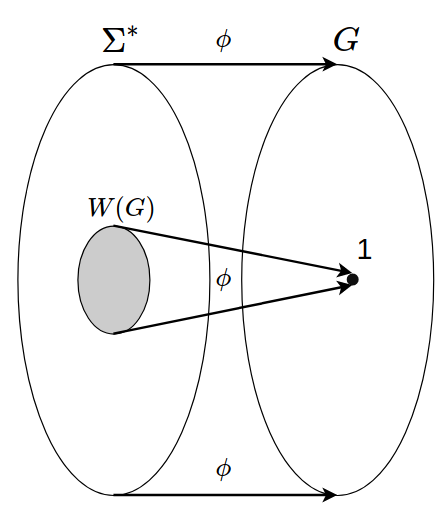
\includegraphics[width=0.6\linewidth]{pics/3.png}}
\caption{Word problem of group.}
\label{fig:word_problem}
\end{figure}

In the following, we present one-tape machine commands that as result replace \eqref{eqreplace},
insert \eqref{eqinsert}, move to left \eqref{eqmove}, move to right \eqref{eqmover} and delete \eqref{eqdelete} squares.

\begin{equation}
    u q v \to u' q' v' \label{eqreplace}
\end{equation}
\begin{equation}
    q \omega \to u q' \omega \label{eqinsert}
\end{equation}
\begin{equation}
    u q \to q' u \label{eqmovel}
\end{equation}
\begin{equation}
    q u \to u q' \label{eqmover}
\end{equation}
\begin{equation}
    u q \omega \to q' \omega \label{eqdelete}
\end{equation}
where $u$, $v$, $u^{'}$, $v^{'}$ are letters, $q$, $q'$ are states.

\subsubsection{Symmetric Turing machine}

In further theorems, a class of Turing machines called symmetric Turing machines will be used. We give definitions that can be seen, for example, in~\cite{symTM}.

\begin{defn}
Turing machine is symmetric if for every command in the set of commands there
is its inverted command.
\end{defn}
For  example, for command
$$u q v \to u' q' v'$$ the inverted command is $$u' q' v' \to u q v$$

\begin{defn}
The symmetrization of a Turing machine $M$ is the symmetric Turing machine $ M^{sym} $ obtained from $M$ by adding the inverse $ \tau^{-1} $ command into a set of commands for each $ \tau $ command from $M$.
\end{defn}

\begin{defn}
Turing machine $M$ is symmetrizable if and only if
$M$ and $ M^{sym} $ are equivalent (i.e. they accept the same language).
\end{defn}

The following theorem is fundamental in the study of the word problem and was obtained
E. Post and A. A. Markov independently of each other in 1947.

\begin{thm} \label{symDetTm}
Every deterministic Turing machine is symmetrizable. On the other hand, not all nondeterministic Turing machines are symmetrizable.
\end{thm}

This means that to obtain an equivalent symmetric machine from a deterministic one, it is enough to simply add inverse commands to the set of commands, but from a nondeterministic one it is not so easy; for this, complex transformations are performed, which will be considered below.

\subsubsection{S-machine}

In addition, the authors introduce a new rewriting system, which they call an S-machine, and define it as follows.

\begin{defn}
Let $n$ be a natural number.
A hardware of an S-machine is a pair $(Y, Q)$ where
\begin{itemize}
    \item $Y$ is a $n$-vector of sets $Y_i$ which elements are called tape letters.
    \item $Q$ is a $(n + 1)$-vector of disjoint sets $Q_i$ which elements are called state letters.
\end{itemize}
The sets of elements of $Q$ and $Y$ are also disjoint.
\end{defn}

With every hardware 
$$S = (Y, Q)$$ 
can be associate the language of admissible words
$$L(S) = Q_1F(Y_1)Q_2 \dots F(Y_n)Q_{n+1}$$
where $F(Y_j)$ is the language
of all reduced group words in the alphabet $Y_j \cup Y_j^{-1}$.

The rewriting rules, or S-rules, have the following form:
$$[U_1 \to V_1, \dots ,  U_m \to V_m]$$
where the following conditions hold:
\begin{enumerate}
    \item Each $U_i$ is a subword of an admissible word starting with a $Q_l$-letter and ending with a $Q_r$-letter.
    \item If $i < j$ then $r(i) < l(j)$.
    \item Each $V_i$ is also a subword of an admissible word whose $Q$-letters belong to $Q_{l(i)} \cup \dots \cup Q_{r(i)}$ and which contains a letter from $Q_l$ and from $Q_r$.
    \item Tape letters are not inserted to the left of $Q_1$-letters and to the right of $Q_{n+1}$-letter.
\end{enumerate}

To apply an S-rule to a word $W$ means to replace simultaneously
subwords $U_i$ by subwords $V_i$, $i = 1, \dots, m$. After every application of
a rewriting rule, the word is automatically reduced.

For example, if a word is
$$q_1 a a q_2 b q_3$$
and the S-rule is
$$[q_1 \to p_1 a^{-1}, q_2 b q_3 \to a^{-1} p_2 b' q_3]$$
where $q_i \in Q_i$, $p_i \in Q_i$, $a \in Y_1$, $b, b' \in Y_2$. Then the result
of the application of this rule is
$$p_1 p_2 b' q_3$$

Besides, with every S-rule $\tau$ we need to associate the inverse S-rule $\tau^{-1}$ in the following way: if
$$\tau = [U_1 \to x_1 V_1 y_1, \dots, U_m \to x_m V_m y_m]$$
then
$$\tau^{-1} = [V_1 \to x_1^{-1} U_1 y_1^{-1}, \dots, V_m \to x_m^{-1} U_m y_m^{-1}]$$

It is worth noting that throughout their work, the authors assume that
an S-machine is symmetric; i. e. if an S-machine contains
a rewriting rule $\tau$, it also contains the rule $\tau^{-1}$.

\subsubsection{The theorems used in the construction}

Earlier all the necessary definitions were given, and further theorems related to them will be presented,
on the evidence of which the algorithm for constructing a presentation of a group by a Turing machine is based.

So, for example, the following theorem states that for any Turing machine $ M $ (including non-deterministic) there is an equivalent symmetric Turing machine, but which is not its symmetrization $ M^{sym} $. That is, to construct an equivalent symmetric Turing machine for any Turing machine, more complex constructions are performed than the simple symmetrization in the Theorem \ref{symDetTm}.
Indeed, Harry R. Lewis and Christos H. Papadimitriou were first who proved a similar theorem~\cite{LEWIS1982161}. The authors modify the construction of such a machine from~\cite{symTM}.

\begin{thm} \label{thmTM}
For any Turing machine $ M $ that recognizes the language $ L $, there is
Turing machine $ M' $ with the following properties:
\begin{enumerate}
\item The language that $ M'$ recognizes is $ L $.
\item $ M'$ is symmetric.
\item A machine accepts a word only when all tapes are empty.
\item Any command $ M' $ or its inverse has one of the following forms for some i:
\begin{IEEEeqnarray}{lCr}
\{q_1\omega \to q_1'\omega, ..., q_{i−1}\omega \to q′_{i−1}\omega, \nonumber
\\ a q_i\omega \to q′_i\omega, q_{i+1}\omega \to q′_{i+1}\omega, ...\}, \label{symType1} \\ \{q_1\omega \to q_1'\omega, ..., q_{i−1}\omega \to q′_{i−1}\omega, \nonumber
\\ \alpha q_i\omega \to \alpha q′_i\omega, q_{i+1}\omega \to q′_{i+1}\omega, ...\} \label{symType2}
\end{IEEEeqnarray}
where $a$ belongs to the tape alphabet of the tape $i$, and $q_j, q'_j$ are the
states of the tape $j$.
\item The letters used on different tapes, including states, belong to non-overlapping alphabets.
\end{enumerate}
\end{thm}

We note that symmetric Turing machines are more similar than usual to a group
because of the possibility of inverse computations that are possible in a group.
The proof of this theorem allows us to construct a symmetric Turing machine
which preserving the recognizable language of the original machine.

In the next step, the authors propose to build an S-machine from a symmetric
Turing machine to achieve even greater similarity with groups.
There is a “natural” way of transforming a Turing machine into an S-machine.
For this, we take a Turing machine $ M $ satisfying all the conditions of Theorem \ref{thmTM},
combine all the tapes of the machine $ M $ and replace each command
$$a q \omega \to q' \omega$$
on 
$$q \omega \to a^{- 1} q' \omega$$
, so the $ M $ commands become S-rules.
Unfortunately, an S-machine constructed in this way does not inherit most
of the properties of the original machine. This is because the S-machine
alphabet contains inverse characters. Therefore, it turns out that
on the one hand, S-machines are much better suited to imitate their work in group relations,
than ordinary Turing machines, since the S-machine can work with reverse alphabet characters (and, moreover, S-machines themselves are considered in \cite{alex2004groups}
as group), and on the other hand, when symmetric Turing machine begins to work as an S-machine, the number of accepted words can increase uncontrollably, since it is possible to recognize negative words.
From this it becomes obvious that in order to preserve a recognizable language, it is necessary to make additional constructions.

Before starting to build an S-machine, the authors make the following renames.
For every $q \in Q$ they denote the word $q \omega$ by $F_q$ and the left marker
on tape $\# i$ by $E_i$.
After renaming a symmetric Turing machine rule
or their inverses have one of the following forms for some $ i $:

\begin{IEEEeqnarray}{lCr} \label{21}
\{F_{q_1} \to F_{q'_1}}, \dots , aF_{q_i} \to F_{q'_i}, \dots , F_{q_k} \to F_{q'_k}\}
\end{IEEEeqnarray}
, where $a \in Y$, or
\begin{IEEEeqnarray}{lCr} \label{22}
    \{F_{q_1} \to F_{q'_1}}, \dots , E_i F_{q_i} \to E_i F_{q'_i}, \dots , F_{q_k} \to F_{q'_k}\}
\end{IEEEeqnarray}

Besides, for any configuration 
$$ C = (E_1 u_1 F_{q_1}, ..., E_k u_k F_{q_k}) $$
of the machine $ M $, they introduce
the value of $\sigma(C)$, which is the admissible word for $S(M)$:

\begin{IEEEeqnarray}{lCr}
E(0)\alpha^n x(0)F(0) \nonumber \\
E(1)u_1x(1)F_{q_1}(1)E'(1)p(1)\delta^{||u_1||}q(1)r(1)s(1)t(1) \nonumber \\
\overline{p}(1)\overline{q}(1)\overline{r}(1)\overline{s}(1)
\overline{t}(1)F'_{q_1}(1) \nonumber \\
... \nonumber \\
E(k)u_k x(k)F_{q_k}(k)E'(k)p(k)\delta^{||u_k||}q(k)r(k)s(k)t(k) \nonumber \\
\overline{p}(k)\overline{q}(k)\overline{r}(k)\overline{s}(k)
\overline{t}(k)F'_{q_k}(k) \nonumber \\
E'(k + 1)x(k + 1)\omega^n F'(k + 1) \nonumber
\end{IEEEeqnarray}
where $n = |u_1| + ... + |u_k|$.

To construct an S-machine equivalent to a symmetric Turing machine, the authors additionally introduce eleven small S-machines (hence the new symbols on tape in the configuration above), which are templates for acceptance management of negative characters. Then, to simulate every rule of a symmetric Turing machine of the form \eqref{21}
start these small S-machines, linking them together with separate S-rules.
And all commands of the form \eqref{22} are matched with one special S-rule.
Thus,
the number of rules in the S-machine is much larger than in the equivalent symmetric Turing machine. 
Here we did not give specific rules for S-machines used in the construction, and additional S-machines, since this takes up a significant part of the article \cite{Sapir} and it makes no sense to rewrite it.
Then the following theorem states that for any Turing machine satisfying Theorem~\ref{thmTM},
there is an S-machine simulating it.

\begin{thm} \label{thmsm}
Let $ M = \langle X, Y, Q, \Theta, s_1, s_0 \rangle $ be a Turing machine,
which satisfies the conditions of Theorem~\ref{thmTM}.
Let $W_0 = \sigma(C_0)$, where $C_0$ is start configuration of the Turing machine $M$.
Then the configuration $ C $ of the machine $ M $ is admissible for $M$ if
and only if $ S (M) $ can transfer $ \sigma(C) $ to $ W_0 $ by rewriting rules.
\end{thm}

At the last step of transforming, the authors finally build the group.
Note that they call one of each pair of mutually inverse rules from $\Theta$
positive and the other negative.
The set of all positive rules is denoted by $\Theta^+$, and the set of
all negative rules is denoted by $\Theta^-$.

\begin{thm} \label{sm2gr}
Let $S(M)$ be the S-machine described in Theorem~\ref{thmsm},
then for any positive integer $N$,
there exists a representation of the group $ G_N (S) $
with the generated set $ A $ and with the set of relations $ P_N (S) $,
where
$$A = \bigcup^{17k+6}_{i=1} Q_i \cup \{\alpha, \omega, \delta\}
\cup \bigcup^k_{i=1}Y_i \cup \{k_j | j = 1, \dots, 2N\} \cup \Theta^+$$
and the set of relationships consists of the following:
\begin{enumerate}
\item Transition relations.

These relations correspond to elements of $ \Theta^+$.
Let $$\tau \in \Theta^+, \tau = [U_1 \to V_1, ..., U_p \to V_p] $$
Then we include the relations 
$$ U^{\tau}_1 = V_1, ..., U^{\tau}_p = V_p $$
If for some $j$ from 1 to $17k + 6$, letters from $Q_j$ do not appear in any of the $U_i$,
then also include the relations 
$$ q^{\tau}_j = q_j $$ 
for each $q_j \in Q_j $.
\item Auxiliary relations.

This is all kinds of relations of the form 
$$\tau x = x \tau $$
, where
$ x \in \{\alpha, \omega, \delta \} \cup^k_{i = 1} Y_i, \tau \in \Theta^+ $ and all relations
of the form 
$$ \tau k_i = k_i \tau$$
, where $i = 1, ..., 2N, \tau \in \Theta^+ $.
\item The hub relation.

Let for each word $u$ denote the word \eqref{eqku}.
\begin{IEEEeqnarray}{rCl}
K(u) &=& (u^{-1} k_1 u k_2 u^{-1} k_3 u k_4 ... u^{-1} k_{2N-1} u k_{2N}) \nonumber \\
&& {} \cdot (k_{2N} u^{-1} k_{2N-1} u ... k_2 u^{-1} k_1 u)^{-1} \label{eqku}
\end{IEEEeqnarray}

Then the hub relation is $K(W_0) = 1$.
\end{enumerate}
\end{thm}

Using this information, we are ready to introduce the main theorem of the considered article.

\begin{thm} \label{basethm}
Let $L \subseteq \Sigma^+$ be the language accepted by the Turing machine $M$, then there exists a finitely presented group $G(M) = \langle A ~ | ~ R \rangle$ and the injective mapping
$$K: \Sigma^+ \to (A \cup A^{-1})^+$$ 
such that: 
$$u \in L \iff K(u) \in W(G)$$
\end{thm}

The authors described and proved all the constructions in the theorems above,
but no one has automated these constructions at the moment,
which we are trying to do in this work.

\section{Implementation}

This section provides a brief description of the algorithm for constructing
a group presentation by a formal context-free grammar.

In this work was used the Haskell functional programming
language\footnote{\url{https://github.com/YaccConstructor/LangToGroup}},
this choice was due to its rich and convenient type system,
which we apply to represent algorithmic types such as formal grammar,
Turing machine, S-machine or group presentation.

The algorithm was divided into modules, each of which
contains the functionality of a specific construction step.
In Fig. \ref{fig:arch} presents the architecture of the algorithm,
where the order of transformation of context-free grammar
into the group presentation is shown. In the picture, types are shown as rectangles with text in the middle, modules are shown as rounded rectangles. The difference in color is due to the belonging of the modules to different groups. Brown unites modules that are responsible for converting types, construction from one type to another. By sequentially applying the functions from these modules, the task of constructing a group presentation by context-free grammar is performed. Purple indicates modules that implement for types the class of printing in LaTeX --- \textit{ShowLaTeX}. They generate the LaTeX code from the types for ease of perception to understand the construction process. Mint denotes interpreter modules that are needed to check the equivalence of transformations in the context of preservation the recognized language during transitions from machine to machine. Green marks additional modules that output the result of computations for further processing using other means. The types and modules of the algorithm will be discussed in detail below.

\begin{figure*}[bp]
\centerline{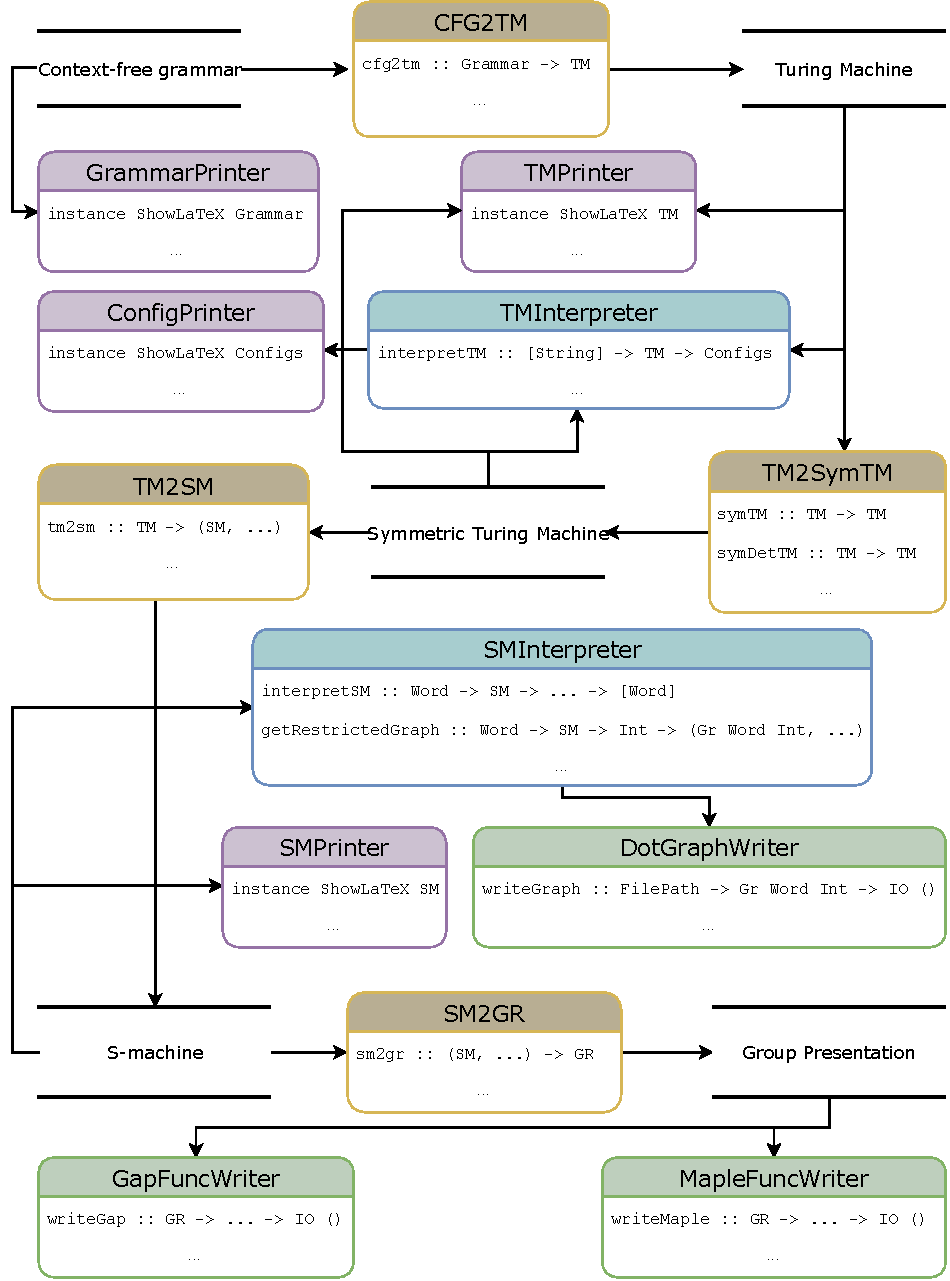
\includegraphics[width=\linewidth]{pics/full_arch(9).pdf}}
\caption{Architecture of the solution}
\label{fig:arch}
\end{figure*}

\subsection{Implemented data types}

In this work, data types of Haskell language were used. Listing \ref{list:types} is a code listing with data types that represent grammars, Turing machines, S-machines, and group presentations, respectively. It is worth noting that data types were intentionally described in the same way as in the definitions of the corresponding concepts. This was done to maintain the maximum similarity to the article.

\begin{listing*}[hbp]
\centering
\begin{minted}{haskell}
-- formal grammar
newtype Grammar = Grammar 
                        (Set Nonterminal, -- set of nonterminals
                        Set Terminal, -- set of terminals
                        Set Relation, -- set of relations
                        StartSymbol) -- start nonterminal
-- Turing machine                        
newtype TM = TM 
                (InputAlphabet, -- input alphabet 
                [TapeAlphabet], -- tapes alphabets
                MultiTapeStates, -- sets of tapes states
                Commands, -- set of commands
                StartStates, -- vector of start states
                AccessStates) -- vector of access states
-- S-machine                
data SM =  SM 
            {yn :: [[Y]], -- tapes alphabets
            qn :: [Set State], -- sets of tapes states
            srs :: [SRule]} -- list of rules
-- group presentation        
newtype GR =  GR 
                (Set A, -- set of generators
                Set GrRelation) -- set of relations
\end{minted}
\caption{Base data types using in the work}
\label{list:types}
\end{listing*}

\subsection{Construction a Turing machine from context-free grammar}

The first part of the algorithm does not connect to the article discussed in the previous section and faced to bridge a gap between context-free grammar and the Turing machine.
To achieve that we implement pushdown automation in terms of the Turing machine we introduced
in the background (see Def. \ref{tm}). The algorithm accepts a formal grammar in Chomsky normal form as input,
it is necessary for ease implementation of pushdown automation.
As mentioned earlier in Theorem ~\ref{thmpda}, it allows us to recognize context-free languages and, finally, with a Turing machine recognizing context-free languages, it is possible to construct a group presentation for context-free languages
(see Theorem ~\ref{basethm}). Thus, within the framework of this work, recognizers for more broad classes of languages that in general a Turing machine can recognize
(e.g., recursively enumerable, Boolean, conjunctive) are not provided, so it is not currently possible for them to build a group presentation. However, for language classes that are subclassed of context-free, it's possible.

The transformation of a context-free grammar into a Turing machine is implemented in the module \textbf{CFG2TM} of the algorithm (see Fig. \ref{fig:cfg2tm}) and can be started using the \textit{cfg2tm} function.

\begin{figure}[H]
\centering
  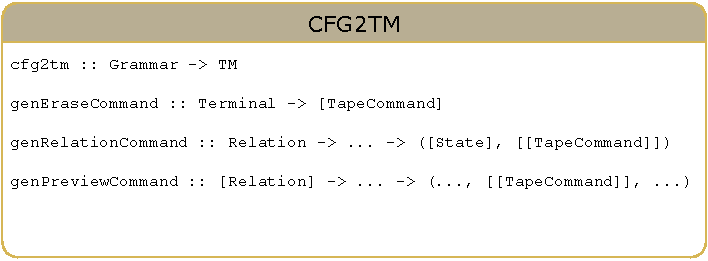
\includegraphics[width=\linewidth]{pics/cfg2tm(1).pdf}
  \caption{Scheme of the module for converting context-free grammar into a Turing machine}
  \label{fig:cfg2tm}
\end{figure}

So, the Turing machine recognizing context-free languages consists of two tapes: the first
tape for the input alphabet, the second for simulating a stack of a pushdown automation.
$\overline{s_1} = (q_0^1, q_0^2)$, $\overline{s_0} = (q_1^1, q_2^2)$ --- vectors of initial and final states respectively.

The first command of the Turing machine places the starting nonterminal on the second tape:
$$\begin{array}{lcl}
    q_0^1 \omega \to q_0^1 \omega \\
    q_0^2 \omega \to S q_1^2 \omega 
\end{array}$$

An accepting command is also introduced, which converts the current state vector of the Turing machine into a vector of final states, if the tapes are empty, that is, if the word was successfully accepted:
$$\begin{array}{lcl}
    \alpha q_0^1 \omega \to \alpha q_1^1 \omega \\
    \alpha q_1^2 \omega \to \alpha q_2^2 \omega 
\end{array}$$

The following commands are grammar dependent and are divided into preview commands, commands generated from grammar rules, and commands received from grammar terminals. Let's consider them in order.

Further, it will be shown that it is advantageous for us to recognize the language if possible by a deterministic Turing machine. There are grammars whose language
can be recognized by a deterministic Turing machine, but by which it is impossible to unambiguously immediately determine which rule should be used. As an example, consider the grammar:
$$\begin{array}{lcl}
    S \to a S b \\
    S \to a b
\end{array}$$ 

Seeing only the letter $ a $ on the tape, it is impossible to determine by one rule which of these two rules should be applied, since the first letter of the right side of the rules is the same. Therefore, rules are generated in the \textit{genPreviewCommand} function that perform previewing one character forward to determine which rule should be applied next. The \textit{genPreviewCommand} function in our example generates the following Turing machine commands:

$\begin{array}{lcl}
    a q_0^1 \to q_2^1 a \\
    S q_1^2 \omega \to S q_1^2 \omega 
\end{array}$,

$\begin{array}{lcl}
    a q_2^1 a \to a q_5^1 a \\
    S q_1^2 \omega \to S q_1^2 \omega 
\end{array}$,
$\begin{array}{lcl}
    b q_2^1 a \to b q_3^1 a \\
    S q_1^2 \omega \to S q_1^2 \omega 
\end{array}$,

$\begin{array}{lcl}
    q_5^1 a \to a q_5^1 \\
    S q_1^2 \omega \to S q_1^2 \omega 
\end{array}$,
$\begin{array}{lcl}
    q_3^1 a \to a q_3^1 \\
    S q_1^2 \omega \to S q_1^2 \omega 
\end{array}$,

$\begin{array}{lcl}
    a q_5^1 \omega \to a q_6^1 \omega \\
    S q_1^2 \omega \to S q_1^2 \omega 
\end{array}$,
$\begin{array}{lcl}
    a q_3^1 \omega \to a q_4^1 \omega \\
    S q_1^2 \omega \to S q_1^2 \omega 
\end{array}$.

Thus, if after the letter $ a $ there is again the letter $ a $, then the first tape of the Turing machine will go to the state $ q_6^1 $, and if there is the letter $ b $, then to the state $ q_4^1 $, and this is how determinism of the Turing machine is obtained by encoding information about the next letter in state.

Next, let's consider what commands of the Turing machine the \textit{genRelationCommand} function generates.
Let the grammar have a rule $ A \to a A'$, then, to simulate this rule,
it is necessary to replace $ A $ on the second tape with symbols from the right side of the rule. Thus, the rule $ A \to a A'$ yields
the following Turing machine commands:

$\begin{array}{lcl}
    a q_0^1 \omega \to a q_0^1 \omega \\
    A q_1^2 \omega \to A' q_3^2 \omega 
\end{array}$,
$\begin{array}{lcl}
    q_0^1 \omega \to q_0^1 \omega \\
    q_3^2 \omega \to a q_4^2 \omega 
\end{array}$,
$\begin{array}{lcl}
    q_0^1 \omega \to q_0^1 \omega \\
    q_4^2 \omega \to q_1^2 \omega 
\end{array}$. 

If the right side of the rule consists of one character, for example, $ A \to a $, then there is no need to generate a new state for writing to the stack, and the following Turing machine command can be generated:

$\begin{array}{lcl}
    a q_0^1 \omega \to a q_0^1 \omega \\
    A q_1^2 \omega \to a q_1^2 \omega 
\end{array}$. 

In the case when the grammar contains a rule in which the right-hand side is an empty word, it is necessary to generate Turing machine commands differently. For example, consider the grammar
$$\begin{array}{lcl}
    S \to \varepsilon \\
    S \to a S b
\end{array}$$
, then for the rule  $S \to \varepsilon$ the \textit{genRelationCommand} function will generate the following Turing machine commands:

$\begin{array}{lcl}
    \alpha q_0^1 \omega \to \alpha q_0^1 \omega \\
    q_0^2 \omega \to S q_1^2 \omega 
\end{array}$,
$\begin{array}{lcl}
    \alpha q_0^1 \omega \to \alpha q_0^1 \omega \\
    S q_1^2 \omega \to q_1^2 \omega 
\end{array}$,
$\begin{array}{lcl}
    b q_0^1 \omega \to b q_0^1 \omega \\
    S q_1^2 \omega \to q_1^2 \omega 
\end{array}$.

The first one pushes $ S $ onto the stack at the start states and an empty input tape, the second applies the rule if the input tape is empty, and the third, if the next character on the tape is $ b $.

Now consider the Turing machine commands that correspond to the grammar terminals and execute
input word acceptance function. For some character of the input alphabet to be recognized
by a Turing machine, it is necessary that it be observed on the input and stack tapes. It is believed that
the Turing machine accepts a certain word if, after the machine is running, its tapes are empty and it is in
final state. Thus, the process of recognizing a character is to erase that character.
from two tapes simultaneously. So, the following command corresponds to any terminal $ a $:

$\begin{array}{lcl}
    a q_0^1 \omega \to q_0^1 \omega \\
    a q_1^2 \omega \to q_1^2 \omega 
\end{array}$. 

The function that maps each terminal to a rule of this kind is called \textit{genEraseCommand}.

Thus, using the functions considered here, the context-free grammar is transformed into a Turing machine that recognizes the language of this grammar. In addition, the Appendix \ref{app:grammar_example} contains an example of building a Turing machine using this algorithm.

\subsection{Symmetrization of the Turing machine}

The next step after constructing a Turing machine is its symmetrization. An equivalent symmetric Turing machine is constructed in the \textbf{TM2SymTM} module (see Fig. \Ref{fig:TM2SymTM}).

In the course of this work, two algorithms for symmetrization of the Turing machine were implemented. One of them is based on the Theorem \ref{thmTM}, which was proved in the article \cite{Sapir}, and the other on the Theorem \ref{symDetTm}. The first algorithm can construct an equivalent symmetric Turing machine for both deterministic and nondeterministic Turing machines. Note that this algorithm in this work is called the symmetrization algorithm for a nondeterministic Turing machine, since deterministic Turing machines are a subclass of nondeterministic ones. The second algorithm can output an equivalent symmetric Turing machine only if a deterministic Turing machine was fed to it, but the size and complexity of the resulting machine is much smaller, what will be shown below. Let's consider these two algorithms.

\begin{figure}[H]
\centering
  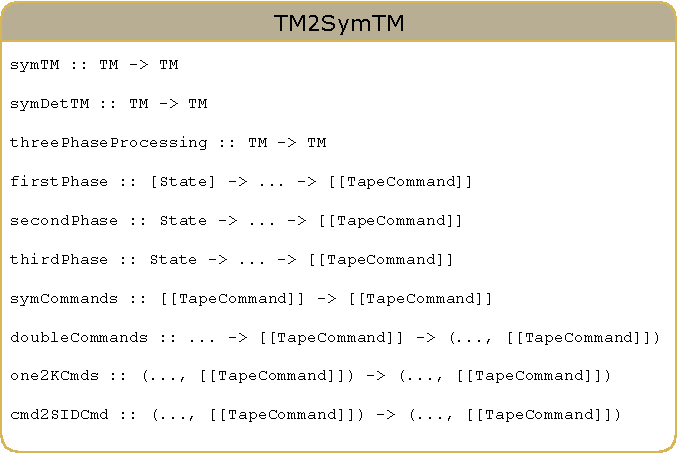
\includegraphics[width=\linewidth]{pics/TM2SymTM(1).pdf}
  \caption{Scheme of the symmetrization module of the Turing machine}
  \label{fig:TM2SymTM}
\end{figure}

\subsubsection{Symmetrization Algorithm for a Nondeterministic Turing Machine}

The entire algorithm can be run with the \textit{symTM} function, which integrates the functions that will be discussed later.

So, the first phase of the algorithm, as in the article \cite{Sapir}, implies the construction of a new Turing machine $ M'$, which is equal to the original one except for the added tape $ k + 1 $, where $ k $ is the number of tapes at the initial machine such that its alphabet consists of the commands of the initial Turing machine. After that, the commands of the Turing machine are generated, which fill the $ k + 1 $ tape non-deterministically, the only restriction here is that the first added command must complete the computation of the original machine. Thus, after the first phase on the $ k + 1 $ tape of the Turing machine $ M '$ there should be a sequence of commands of the original Turing machine, where the first command completes its computation (transforms the state vector into the vector of final states). After that, the transition to the second phase occurs.

The second phase is that $ M'$ tries to execute commands in the order in which they appear on the $ k + 1 $ tape. To do this, from the command of the original Turing machine:
$$\tau = \{ U_1 \to V_1, ... , U_k \to V_k \}$$
following command of $ M'$ is being built:
$$\tau' = \{ U_1 \to V_1, ... , U_k \to V_k, \tau q \to q \tau \}$$
where $ q $ is the state of $ M'$ on the tape $ k + 1 $.

The authors claim that after such calculations, the first tape $ M '$ will be empty, and $ k + 1 $ on the right will observe $ \alpha $ only if, during the first phase, a sequence of commands of the original Turing machine was written on the $ k + 1 $ tape, which brings it to its final states.

After the second phase, $ M '$ returns the head to $ \omega $ on the $ k + 1 $ tape and the third phase begins, which consists in clearing all the tapes and transitioning to the vector of final states.

These three phases are implemented in functions with the corresponding names \textit{firstPhase}, \textit{secondPhase}, \textit{thirdPhase}, and the \textit{threePhaseProcessing} function integrates them and builds $ M '$ after these three phases, at the end of this paper in the Appendix \ref{app:tm_example}, you can see the result of this function on a Turing machine from one rule.

As stated in \cite{symTM}, it is now possible to construct an equivalent symmetric Turing machine from $ M'$ by adding its inverse to the set of commands for each command. In the algorithm, this is done by the \textit{symCommands} function.
Thus, after these steps $ M '$ satisfies the first three properties from the \ref{thmTM} theorem, and it remains to transform it so that it satisfies the last two properties.

To achieve the fourth property, the tapes are doubled. So for any tape $ i $ there appears a tape $ i + 1/2 $, such that if the initial configuration of the tape $ i $ is $ \alpha uqv \omega $, then after doubling the configuration of the tapes $ i $ and $ i + 1/2 $: $ \alpha uq \omega $ and $ \alpha \Bar{v} q \omega $, respectively, where $ u, v $ are words, $ \Bar{v} $ is $ v $, written from right to left, $ q $ state, which is further renamed to achieve property 5. In this regard, it is necessary to replace every command:
$$\{ u_1 q_1 v_1 \to u_1' q_1' v_1',  ... , u_k q_k v_k \to u_k' q_k' v_k' \}$$
to the command:
\begin{center}
    $\{ u_1 q_1 \omega \to u_1' q_1' \omega, \Bar{v_1} q_1 \omega \to \Bar{v'_1} q_1' \omega , ... , \newline
    u_k q_k \omega \to u_k' q_k' \omega, \Bar{v_k} q_k \omega \to \Bar{v'_k} q_k' \omega \}$
\end{center}

If $ v $ in any of the commands is equal to $ \omega $, then $ \Bar{v} = \alpha $. Obviously, a Turing machine that is transformed in this way will recognize the same language as the original Turing machine. These conversions are implemented in the \textit{doubleCommands} function.

The next step is to split each command into $ 2k $ commands so that each new command affects only one tape. This operation is performed in the \textit{one2KCmds} function. To this end, many unique states are generated for each command to maintain the order of computation. Thus, the following commands are obtained:
$$\{ q_1 \omega \to q_1' \omega , ... , u_i q_i \omega \to u_i' q_i' \omega , ... \}$$

Note that if $ u_i = \alpha $, then the command already has the form \eqref{symType2}, since $ u_i '$ is also equal to $\alpha $, otherwise you need to double the command again so that they look like \eqref{symType1} and this is done by the \textit{cmd2SIDCmd} function:
$$\{ q_1 \omega \to q_1'' \omega , ... , u_i q_i \omega \to q_i'' \omega , ... \}$$
$$\{ q_1'' \omega \to q_1' \omega , ... , q_i'' \omega \to u_i' q_i' \omega , ... \}$$

Thus, a Turing machine is constructed that satisfies 4 property of the Theorem \ref{thmTM}. To satisfy property 5, it is enough to generate unique names for states and letters, which happens in the algorithm during the construction process.

\subsubsection{Symmetrization Algorithm for a Deterministic Turing Machine}

Note that the first three phases of the symmetrization algorithm of a nondeterministic Turing machine are aimed at building an equivalent symmetric Turing machine and, if we have an alternative version of its construction, these actions can be omitted.

As it was written above, according to the Theorem \ref{symDetTm} it is possible to get an equivalent symmetric Turing machine from a deterministic Turing machine by simply adding its inverse to the set of commands for each command. But properties 4 and 5 of Theorem \ref{thmTM} still need to be provided in a symmetric machine in order to proceed to the next step of constructing a group presentation.
Therefore, to successfully build an equivalent symmetric Turing machine based on a deterministic Turing machine, it is sufficient to execute the \textit{symDetTM} function, which integrates the \textit{doubleCommands}, \textit{one2KCmds}, \textit{cmd2SIDCmd} and \textit{symCommands} functions, discussed above and guaranteeing the execution of properties 4 and 5. In addition, in the Appendix \ref{app:tm_example}, you can see an example of how the algorithm works.

\subsection{Construction of an S-machine from a symmetric Turing machine}

In this subsection, we will consider an algorithm for constructing an S-machine that simulates a symmetric Turing machine and, in a sense, preserves the language recognized by this Turing machine. The module, which implements the functions necessary for construction, is called \textbf{TM2SM}, and its diagram is shown in Fig. \ref{fig:TM2SM}. The function that constructs the S-machine is called \textit{tm2sm}, further we consider the functions, the superposition of which it is.

\begin{figure}[H]
\centering
  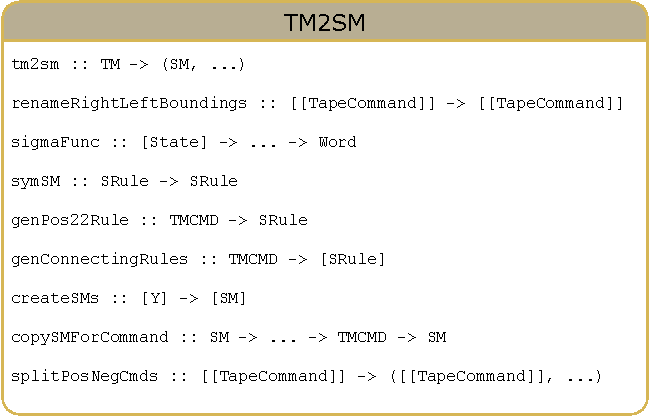
\includegraphics[width=\linewidth]{pics/TM2SM(2).pdf}
  \caption{Diagram of a module of constructing an S-machine that simulates a Turing machine}
  \label{fig:TM2SM}
\end{figure}

As it was already mentioned in the background section, before immediately building the S-machine, the instructions of the Turing machine are renamed so that they have one of the forms \eqref{21}, \eqref{22}. This action in this work is performed by the \textit{renameRightLeftBoundings} function. Also, 11 auxiliary S-machines are built in the \textit{createSMs} function: $ S_1 $, $ S_2 $, $ S_3 $, $ S_4 $, $ S_5 $, $ S_6 $, $ S_7 $, $ S_8 $, $ S_9 $ , $ S_{\alpha} $, $ S_{\omega} $, and S-rules are generated in the \textit{genConnectingRules} function, which are transitional between auxiliary machines.

After that, each command of a Turing machine of the form \eqref{21} is matched with a set of S-rules of auxiliary S-machines and transitional S-rules, and all commands of the form \eqref{22} are matched with one S-rule that does not perform calculations but changes state. The matching is done by adding to the S-rules a label of a particular Turing machine command.

The search for commands of the form \eqref{21}, \eqref{22} is performed by the \textit{splitPosNegCmds} function, the comparison of sets of S-rules to a command of the form \eqref{21} is performed by the function \textit{copySMForCommand}, and the generation of S- rules for a command of the form \eqref{22} function \textit{genPos22Rule}.
In addition, the S-machine symmetrization function \textit{symSM} and the $ \sigma(C) $ (\textit{sigmaFunc}) function, the meaning of which was described in the background, are implemented.

The states of the resulting S-machine are all the states of the labeled auxiliary S-machines, combined with all also labeled $ E_i $ and $ F_q $, which were obtained after renaming the Turing machines, where $ i = 1..k $ is the tape number, $ q \in Q $ state of the Turing machine.
The S-machine alphabet are the combined alphabets of the auxiliary S-machines with the Turing machine alphabet.

\subsection{Constructing a Group Presentation from an S-Machine}

The process of constructing a group representation on an S-machine has been described in detail in Theorem \ref{sm2gr}. In this subsection, we'll show you what functions do this build.
\textbf{SM2GR} --- the module that contains these functions (see Fig. \ref{fig:SM2GR}).

\begin{figure}[H]
\centering
  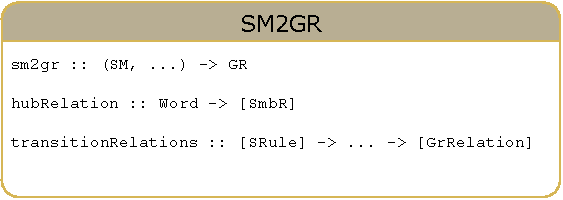
\includegraphics[width=\linewidth]{pics/SM2GR(1).pdf}
  \caption{Diagram of a module of constructing a group presentation by an S-machine}
  \label{fig:SM2GR}
\end{figure}

Transitional, auxiliary relations and the hub relation are generated in the \textit{transitionRelations}, \textit{auxiliaryRelations} and \textit{hubRelation} functions, respectively. Genertors of the group presentations are forming in the \textit{sm2gr} function, which also unifies all relations.

\subsection{Supporting tools}

The subsection describes additional modules of the application developed in this work, which were written, firstly, in order to facilitate perception and, secondly, to test the equivalence of transformations in the context of preserving the recognized language during transitions from machine to machine and which can be seen above in Fig. \ref{fig:arch}.

For the first, modules were developed that generate LaTeX code, with the ability to generate it for displaying grammars, Turing machines, configurations of Turing machines, S-machines.
For this generation, the HaTeX\footnote{HaTeX is a library that implements LaTeX syntax and several useful abstractions.

Library description: \url{https://hackage.haskell.org/package/HaTeX-3.22.2.0}

Date of last visit: 14.05.20} library was used. The \textit{ShowLaTeX} class was created and implemented for all types that needed to be printed in LaTeX.
Thus, modules in the Haskell language \textbf{GrammarPrinter}, \textbf{TMPrinter}, \textbf{SMPrinter} and \textbf{ConfigPrinter} were implemented, in which the \textit{ShowLaTeX} class is implemented for the \textit{Grammar}, \textit{TM}, \textit{SM} and \textit{Configs} respectively. Examples of this generation can be seen in the Appendix \ref{app:grammar_example} and \ref{app:tm_example}.

For the second, modules were written that interpret Turing machines and S-machines separately on given input data, the general concept of which is breadth-first search of the configuration tree with the stopping if the final configuration is in the front set. So, when traversing in breadth-first, to each configuration from the front, it is necessary to apply the commands of the Turing machine or S-rules that can be applied to this configuration, and the resulting configurations, after application, add to the front set.

Such breadth-first traversal works well in the case of a Turing machine, and in the S-machine interpreter, due to its strong non-determinism, a set was also used in which the traversed configurations are stored. If, after applying the rule, the resulting configuration is already in this set, then such a configuration is not added to the front. This eliminates the possibility of returning to the configurations already passed, which makes it easier to find the final configuration.

The result of the work of the interpreters is the history of the passed configurations, which led to the final one and from which LaTeX can be generated if necessary.

The functions for interpreting the Turing machine are contained in the \textbf{TMInterpreter} module, where the \textit{interpretTM} function performs the interpretation. Similarly, the S-machine interpreter module \textbf{SMInterpreter}, where \textit{interpretSM} interprets.
In addition, this module contains the \textit{getRestrictedGraph} function, which builds a graph of a given height. This graph can then be printed to a dot file using the \textit{writeGraph} function of the \textbf{DotGraphWriter} module, which prints it using the Graphviz\footnote{Graphviz is an open source graph rendering toolkit.

Library description: \url{https://hackage.haskell.org/package/graphviz}

Date of last visit: 14.05.20} library.

In addition, \textbf{GapFuncWriter} and \textbf{MapleFuncWriter} modules were implemented that have \textit{writeGap} and \textit{writeMaple} functions which print the group presentation into the source file of the mathematical packages GAP\footnote{GAP (Groups, Algorithms, Programming) is a software package, an open source computer algebra system with a special emphasis on computational group theory.

Package site: \url{https://www.gap-system.org/}

Date of last visit: 14.05.20} and Maple\footnote{Maple is a software package, a computer mathematics system focused on complex mathematical calculations, data visualization and modeling.

Package site: \url{https://www.maplesoft.com/products/Maple/}

Date of last visit: 14.05.20} respectively, for further analysis of the groups presentations by them.

Thus, we have the opportunity to visually demonstrate the result of the algorithm and check whether the recognized languages match after transitions.

\section{Evaluation}

This section presents the results of the pipeline execution of algorithms for constructing a presentation of a group from context-free grammars in Chomsky normal form with the derivation of the numerical sizes of machines at all transformation steps.
    
To estimate the size of the resulting group presentation, we ran
algorithms with non-deterministic and deterministic
symmetrization on three grammars: one rule grammar \eqref{eqonerule},
grammar of "a*" language \eqref{eqastar} and unambiguous grammar of Dick language on one type of brackets \eqref{eqdyck}.

\begin{multicols}{2}
\noindent
\centering
    \begin{IEEEeqnarray}{lCr}
        \nonumber \\ S \to a \label{eqonerule}
    \end{IEEEeqnarray}
    \begin{IEEEeqnarray}{lCr}
        S \to AS ~|~ \varepsilon \label{eqastar} \\
        A \to a \nonumber
    \end{IEEEeqnarray}
    \begin{IEEEeqnarray}{lCr}
        S \to AC ~|~ \varepsilon \nonumber \\
        C \to SD \nonumber \\
        D \to BS \label{eqdyck} \\
        A \to a \nonumber \\
        B \to b \nonumber
    \end{IEEEeqnarray}
\end{multicols}

Table \ref{tab:1} shows the sizes of each of the sets of our algebraic types, built in the process of the algorithm with nondeterministic symmetrization of the Turing machine. It is obvious from it that an algorithm was obtained that builds a rather large presentation of the group even on simple initial data. So, grammar from just one rule turns into about 90 thousand group relations and 56 thousand generators.

\begin{table*}[b]
\begin{center}
\begin{tabular}{|c!{\vrule width 1pt}
c|c|c!{\vrule width 1pt}
c|c|c|c!{\vrule width 1pt}
c|c|c|c!{\vrule width 1pt}
c|c|c!{\vrule width 1pt}
c|c!{\vrule width 1pt}}
\hline
&
\multicolumn{3}{|c|}{\textbf{Grammar}}&
\multicolumn{4}{|c|}{\textbf{TM}}&
\multicolumn{4}{|c|}{\textbf{TM'}}&
\multicolumn{3}{|c|}{\textbf{SM}}&
\multicolumn{2}{|c|}{\textbf{G}}\\
\cline{2-17}
&$\Sigma$&$N$&$R$
&$X$&$\Gamma$&$Q$&$\Theta$
&$X$&$\Gamma$&$Q$&$\Theta$
&$Y$&$Q$&$\Theta$
&$A$&$R$\\
\hline
1 rule
&1&1&1
&1&3&5&4
&1&14&270&206
&14&88246&2363
&89508&56187\\
\hline
$a^*$
&1&2&3
&1&4&7&9
&1&26&547&434
&26&344118&5741
&347370&204903\\
\hline
Dyck
&2&4&6
&2&8&11&19
&2&54&1131&900
&54&1469136&15064
&1478859&957619\\
\hline
\end{tabular}
\end{center}
\caption{Cardinalities of sets of machines when using the symmetrization algorithm of nondeterministic Turing machines}\label{tab:1}
\end{table*}

But analyzing this table, you can see that the main growth in size occurs at the stages of symmetrization of the Turing machine and transformation of the symmetric Turing machine into an S-machine. Therefore, in order to reduce the size of the symmetric Turing machine, the symmetrization algorithm of the deterministic Turing machine was implemented, which is also discussed above. The Table \ref{tab:2} shows the results of its work.

\begin{table*}[b]
\begin{center}
\begin{tabular}{|c!{\vrule width 1pt}
c|c|c!{\vrule width 1pt}
c|c|c|c!{\vrule width 1pt}
c|c|c|c!{\vrule width 1pt}
c|c|c!{\vrule width 1pt}
c|c!{\vrule width 1pt}}
\hline
&
\multicolumn{3}{|c|}{\textbf{Grammar}}&
\multicolumn{4}{|c|}{\textbf{TM}}&
\multicolumn{4}{|c|}{\textbf{TM'}}&
\multicolumn{3}{|c|}{\textbf{SM}}&
\multicolumn{2}{|c|}{\textbf{G}}\\
\cline{2-17}
&$\Sigma$&$N$&$R$
&$X$&$\Gamma$&$Q$&$\Theta$
&$X$&$\Gamma$&$Q$&$\Theta$
&$Y$&$Q$&$\Theta$
&$A$&$R$\\
\hline
1 rule
&1&1&1
&1&3&5&4
&1&6&39&34
&6&6058&501
&6410&7637\\
\hline
$a^*$
&1&2&3
&1&4&7&9
&1&8&73&72
&8&15888&1024
&16565&17657\\
\hline
Dyck
&2&4&6
&2&8&11&19
&2&16&161&158
&16&67754&2837
&69772&71533\\
\hline
\end{tabular}
\end{center}
\caption{Cardinalities of sets of machines using the symmetrization algorithm of deterministic Turing machines}\label{tab:2}
\end{table*}

Note that, indeed, the use of this algorithm reduced the size of the symmetric Turing machine, the S-machine, and the group presentation by several times in comparison with the use of the symmetrization algorithm for nondeterministic Turing machines. It is clear that the smaller the group presentation, the easier it is to find words that are equal to the group unit. From this we can conclude that in the case of deterministic grammars, one should use symmetrization for deterministic machines.

Attempts were also made to check for equality to groups' unit some words from the obtained groups presentations using the mathematical packages GAP and Maple. Unfortunately, due to the complexity of the calculations, the mathematical packages with which the experiments were carried out did not complete their work in an acceptable time.

\section{Conclusion}

During this work, an algorithm for transforming a context-free grammar into a Turing machine of a special notation was implemented, on the basis of the article \cite{Sapir} an algorithm for constructing a group presentation by a Turing machine was developed, interpreters for a Turing machine and an S-machine were developed, and a number of construction experiments were carried out, which showed advantages of using the algorithm of deterministic symmetrization of Turing machines.

Since the described solution does not currently have its application, there is a need to improve it, namely, if you want to get a presentation of a group of satisfactory sizes, then in further work it is necessary to find out how to transform symmetric Turing machines into S-machines in a more optimal way.

We can argue that it is possible to find a more optimal algorithm for constructing an S-machine from a symmetric Turing machine for a number of reasons.
Firstly, there are alternative ways of constructing an S-machine from the symmetric Turing machine \cite{SpaceFunc}.
Secondly, since some languages can be used to construct a group presentation, for example, for the language $ L = \{a\} $, we can construct a group presentation and a relation from the Theorem \ref{basethm} such that
$$ G = \langle k_1, k_2, a ~|~ k_1 a k_2 = 1 \rangle $$
and $ K (a) = k_1 a k_2 $. It is clear that such a construction works only for finite languages, but this suggests the idea that, perhaps, there is a simpler construction in the general case.

In addition, the question of interpreting the group's presentation remains relevant, since the existing mathematical packages could not cope with this task.

\begin{appendices}

\section{Transformation of the grammar} \label{app:grammar_example}

This section provides an example of the work of the above algorithm for converting the elementary grammar into a Turing machine with its subsequent interpretation.

From the following one-rule grammar:
\subfile{examples/1rg.tex}

The following Turing machine was obtained using the algorithm implemented in the framework of this work:
\subfile{examples/1rgtm.tex}

At this point let's explain the notation of the commands. Every Turing machine command is enclosed in square brackets, where each line represents the single-tape Turing machine command that belongs to the corresponding tape. The single-tape Turing machine command has been announced above and in the article \cite{Sapir}. Looking at one of the commands above, you can understand that they refer to a Turing machine with two tapes, and on the first line of the command is a single-tape command related to its first tape, and on the second to the second tape. Thus, the line number corresponds to the tape number of the Turing machine.

Then we interpreted the resulting Turing machine on the input line $ a $ and got the history of configuration changes:
\subfile{examples/1rgtmconfg.tex}

\section{Transformation of the Turing machine} \label{app:tm_example}

In this section, an example of the operation of three phases of the symmetrization algorithm for non-deterministic Turing machines, namely the \textit{threePhaseProcessing} function, and also the symmetrization algorithm for a deterministic Turing machine, is considered.

From a Turing machine containing one rule and accepting a language from one word $ a $:
\subfile{examples/1rtm.tex}

After three phases of symmetrization by the algorithm for nondeterministic machines, we obtain a symmetric Turing machine that does not satisfy the 4th property of the Theorem \ref{thmTM}:
\subfile{examples/1rtm3phase.tex}

You can notice that in the example above, the Turing machine commands are used as symbols on the last tape, the introduction of such a tape is necessary to symmetrize the nondeterministic Turing machine. Here, you should think of commands within a command as simple symbols on the tapes that you can replace, move, add, and remove. They themselves no longer perform the function of commands but are simply symbols that indicate belonging to a particular command. With the same success, it was possible to use any other characters for a similar encoding of a symbol's belonging to a command, but we decided that it would be more descriptive.

And applying the symmetrization algorithm of a deterministic Turing machine to the same elementary machine, we obtain a symmetric Turing machine:
\subfile{examples/1rtmsym.tex}

Unfortunately, the size of S-machines does not allow us to give an example of their construction here, but printing S-machines is possible. Similarly, we cannot give here even the smallest example of transforming a grammar into an S-machine with the inference of intermediate Turing machines. It will take a lot of pages, but you can repeat the experiments yourself, and print it to LaTeX by command-line flags, which are been implemented for this, examples of its use you can find in the readme\footnote{\url{https://github.com/YaccConstructor/LangToGroup/blob/master/README.md}}.

\end{appendices}

\bibliographystyle{IEEEtran.bst}
\bibliography{IEEEbib.bib}
\end{document}
